\documentclass[12pt, a4paper]{article}
\usepackage{graphicx}
\usepackage{mathtools}
\usepackage{amsmath}
\usepackage{geometry}
\linespread{1.1}
\usepackage{caption}
\usepackage[italian]{babel}

\geometry{
 total={170mm,257mm},
 left=20mm,
 top=15mm,
 bottom=28mm
 }
\title{\textbf{\scalebox{1.4}{\text{{\Huge Pendolo}}}}}
\date{}
\author{\begin{small}Mussini Simone, Ruscillo Fabio, Musi Francesco\end{small}}
\begin{document}
\maketitle



\section{Richiami teorici}
La molla è un corpo elastico, capace di deformarsi se viene applicata una forza e di tornare sempre allo stesso allungamento in condizioni di equlibrio. 
Poichè tende a ritornare alla sua posizione di equilibrio, quando deformata esercita una forza, che segue la \textit{Legge di Hooke}: 

\begin{equation}
    F_{el} = -K(X-X_0)
\end{equation}

Dove $X-X_0$ è la deformazione linare, $K$ è la costante elastica propria di ogni molla e il segno meno 
indica che è una fornza di richiamo, in direzione opposta alla forza esterna applicata.
In condizioni ideali, quindi senza forze dissipative, l'equazione del moto di una molla è quella di 
un oscillatore armonico con pulsazione $\omega = \sqrt{\frac{K}{m}}$ ($m$ = massa del corpo collegato alla molla, la massa della molla è trascurabile). La soluzione dell'equazione differenziale è una funzione sinusoidale con ampiezza $A$ e fase iniziale $\phi$:

\begin{equation}
    F_el = m\ddot{x} = -Kx   \quad\xrightarrow{}\quad   \frac{d^2x}{dt^2} = -\omega^2x  \quad\xrightarrow{}\quad   x(t) = A cos(\omega t + \phi)
\end{equation}

Il periodo di una oscillazione risulta: $T = \frac{2\pi}{\omega} = 2\pi\sqrt{\frac{m}{K}}$.


\section{Obbiettivi}
Gli obbiettivi di questo esperimento sono: 
Determinare la costante elastica di una molla $(K_s)$ con metodo statico,  utilizzare la molla come dinamometro statico per la determinazione di una massa incognita $(M_i)$, per determinare la costante elastica di una molla precompressa $(K_p)$ e la forza di precompressione con il metodo statico $(F_0)$.


\section{Strumenti}
    \begin{itemize}
        \item Masse calibrate
        \item Massa ignota 
        \item Molla armonica   
        \item Molla precompressa 
        \item Metro a nastro 
        \item Cronometro 
        \item Sostegno fisso 
    \end{itemize}

    
\section{Procedimento}
Il setup dell'esperimento è costituito da un piedistallo, la cui funzione è di sostenere due aste, collegate tra loro tramite un morsetto, in modo da formare un supporto per sostenere le molle in posizione verticale.
All'asta messa in orizzontale rispetto al piano, del tavolo, viene poi fissato un metro a nastro, al fine di misurare le deformazioni, che verranno indotte sulle molle. 



\section{Analisi preliminare}
Per avere una stima sull'ordine di grandezza dell'errore su $K_s$, si è calcolato l'errore relativo della costante elastica della molla, in modo statico, tramite singola misura, usando la formula 
\begin{equation*}
    \frac{\Delta K_s}{K_s}=\frac{\Delta M}{M}+\frac{\Delta g}{g}+ \frac{\Delta (L-L_0)}{L-L_0}
\end{equation*}

Si è calcolata la lunghezza della molla a riposo e in seguito quella della molla deformata da una massa di $m=250$ $g$.
Si è assunta quest'ultima e l'accelerazione di gravità $g$ senza incertezza, in modo da avere una stima preliminare dell'ordine di grandezza dell'errore.
Dato l'allungamento $(L-L_0)=0.095\pm 0.005$ $m$ l'errore relativo au $K_s$ è circa il $6$\%.

Per la stessa ragione, si è calcolato l'errore relativo della costante elastica della molla, in modo dinamico, tramite singola misura, usando la formula 
\begin{equation*}
    \frac{\Delta K_d}{K_d}=\frac{\Delta M}{M}+2\frac{\Delta T}{T}
\end{equation*}
Per avere un errore relativo minore, si è calcolato il periodo di dieci oscillazioni, pari a $10T= 9,30 \pm 0.1$ $s$  GAUSSIANA CON CLASSI + TEST CHI QUADRO. Inserendo nella fomrula $\overline T$, il il valore medio diviso per dieci, otteniamo un errore relativo su $K_d$ del 2 \%.



\section{Misura della costante elastica con il metodo statico}
Questo step consiste nel misurare l'allungamento delle due molle soggette a differenti forze, generate dai contrappesi. I dati sono riportati di seguito in Tabella \ref{tab: Misure Statiche Non Precompresse} e Tabella \ref{tab: Misure Statiche Precompresse}:
\\

\begin{table}[!htb]
    \begin{minipage}[t]{.5\linewidth}
    \centering
        \begin{tabular}{|c|c|}
        \hline
        $M$ $(kg)$&$L\pm \Delta L$ $(m)$\\
        \hline
        $0.050$ & $0.326$$\pm$$0.002$\\
        $0.100$ & $0.346$$\pm$$0.002$\\
        $0.150$ & $0.366$$\pm$$0.002$\\
        $0.200$ & $0.387$$\pm$$0.002$\\
        $0.250$ & $0.407$$\pm$$0.002$\\
        $0.300$ & $0.427$$\pm$$0.002$\\
        $0.350$ & $0.448$$\pm$$0.002$\\
        $0.400$ & $0.468$$\pm$$0.002$\\
        $0.450$ & $0.489$$\pm$$0.002$\\
        $0.500$ & $0.509$$\pm$$0.002$\\
        \hline
    \end{tabular}
    \captionsetup{width=7cm}
    \caption{Molla Non Precompressa. Sono riportati la massa e la posizione finale misurata in seguito alla deformazione.}

    \label{tab: Misure Statiche Non Precompresse}
    \end{minipage}
    \begin{minipage}[t]{.5\linewidth}
    \centering
        \begin{tabular}{|c|c|}
            \hline
            $M$ $(kg)$&$L\pm \Delta L$ $(m)$\\
            \hline
            $0.050$ & $0.203$$\pm$$0.003$\\
            $0.100$ & $0.203$$\pm$$0.003$\\
            $0.150$ & $0.203$$\pm$$0.003$\\
            $0.200$ & $0.208$$\pm$$0.003$\\
            $0.250$ & $0.224$$\pm$$0.003$\\
            $0.300$ & $0.242$$\pm$$0.003$\\
            $0.350$ & $0.259$$\pm$$0.003$\\
            $0.400$ & $0.276$$\pm$$0.003$\\
            $0.450$ & $0.295$$\pm$$0.003$\\
            $0.500$ & $0.313$$\pm$$0.003$\\
            \hline
        \end{tabular}
        \captionsetup{width=7cm}
        \caption{Molla Precompressa. Al di sotto di una massa pari a $0.150$ $kg$ non si è ossservata alcuna deformazione della molla.}
        
        \label{tab: Misure Statiche Precompresse}
    \end{minipage} 
\end{table}






\subsection{Molla Armonica (non precompressa) - metodo statico}
Dato che la legge di Hook $Mg=K_s\cdot(L-L_0)$ ci suggerisce che l'allungameto sia in relazione lineare con la forza applicata, abbiamo attuato una regressione lineare. 
Per la molla non precompressa la legge di cui trovare i coefficienti è: 
\begin{equation*}
    L=M\cdot\displaystyle\frac{g}{K_s}+L_0
    \xrightarrow{} Y = A + BX
\end{equation*} 
dove\\ 
\begin{equation*}
 A= L_0 \mbox{ , } B=\displaystyle\frac{g}{K_s} \mbox{ , } y = L \mbox{ e } X = m
\end{equation*}



\begin{figure}[h]
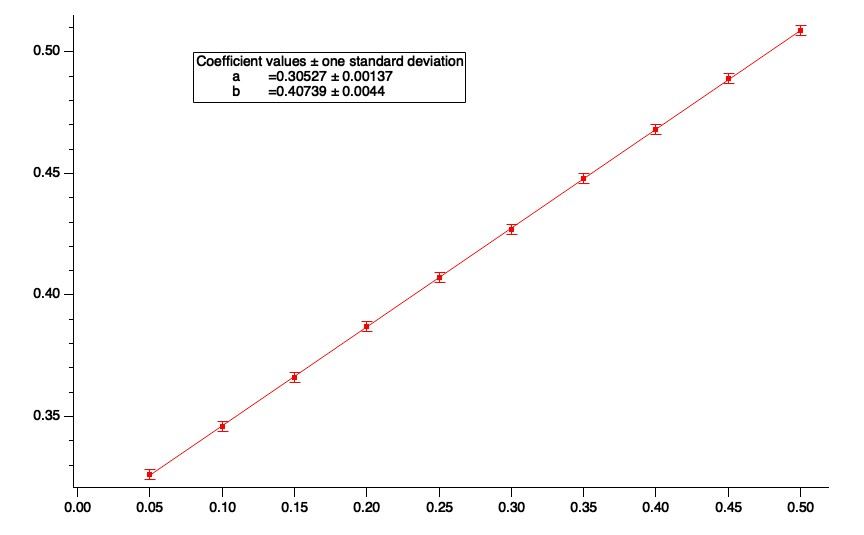
\includegraphics[width=170mm]{IMMAGINI/Graph Molla Arm Stat.jpg}
\centering
\caption{\textit{{\footnotesize{Grafico $L(M)$}: sul'asse asse \textit{y} sono riportati i valori della posizione finale misurata $L$ coi rispettivi errori, sull'asse \textit{x} la massa corrispettiva}}}
\label{Grafico parabolico}
\end{figure}


\bigskip
\bigskip


Calcolando $K_s$ e il rispettivo errore $\Delta K_s$ come\\

\begin{equation*}
\centering
    K_s= \frac{g}{B} \text{\phantom{Testo invi}} \text{,} \text{\phantom{Testo sibil}} \Delta K_s = \left | \frac{g}{B}  \right | \cdot \Delta B 
\end{equation*}
\bigskip

Si ottiene $K_s = (24.1 \pm 0.2)$ $N m^{-1}$






\subsection{Molla Precompressa - metodo statico}
Nel caso di una molla precompressa, la legge che lega l'allungamento alla forza applicata differisce dalla legge di Hooke per un termine costante $\frac{F_0}{K_p}$ , dovuto alla forza $F_0$ di precompressione della molla.  
\\La legge su cui abbiamo eseguito la regressione lineare risulata quindi: 
\begin{equation}
    L = m \frac{g}{k_p} + (L_0 - \frac{F_0}{K_p}) 
\end{equation}
dove 
\begin{equation}
    A = L_0 + \frac{F_0}{K_p} \  \ \ \   e   \ \ \ \ B = \frac{g}{K_p}
\end{equation}
\\Calcolando $K_p$ e il rispettivo errore $\Delta K_p$ come : 
\begin{equation}
    K_p = \frac{g}{B} e \Delta K_p = \left | \frac{g}{B}  \right | \cdot \Delta B 
\end{equation}






\section{Misura della costante elastica con metodo dinamico }
Questo step consiste nel misurare il tempo impiegato dalla molla, alla quale è fissato un pesetto da $500kg$, a compiere dieci oscillazioni complete. Al fine di ricavare la costante $k_d$ dalla relazione: 
\begin{equation}
    T = 2\pi \cdot \sqrt{\frac{k_d}{m}}
\end{equation} 

Per avere una miglior stima del periodo, abbiamo misurato 30  volte il tempo relativo alle 10 oscillazioni, inserendoli con le relative frequenze di misura, nella Tabella \ref{tab: Misure Dinamiche} a fine paragrafo.  

Abbiamo controllato che il campione fosse compatibile con una distribuzione gaussiana.
Calcolando il valore medio $\overline{x}$ e la deviazione standar $\sigma_x$ tramite le formule: 
\begin{equation}
    \overline{x} = \frac{\sum_{i=1}^{N}x_i}{N} \mbox{\hspace{0.5cm} , \hspace{0.5cm}}
    \sigma_x = \sqrt{\frac{\sum_{i=1}^{N}(x_i-\overline{x})^2}{(N-1)}}
\end{equation}

\smallskip
Nel nostro caso $\overline{x} = 9,2773$ e $\sigma_x = 0,0921 $. 
Ora possiamo dividere le misure delle dieci oscilazioni in classi con il relativo numero valori osservatie  riportarle  nella seguente tabella  


\begin{table}[hbt!]
    \centering
    {\renewcommand\arraystretch{1.0} 
    \begin{tabular}{|c|c|}
    \hline
        \textbf{Dieci Periodi} & \textbf{Frequenza}\\
        $10T(s)$ & $f(n)$\\
    \hline
    $ 9.07 $ & $ 1 $ \\ 
    $ 9.12 $ & $ 1 $ \\
    $ 9.13 $ & $ 1 $ \\
    $ 9.15 $ & $ 1 $ \\ 
    $ 9.21 $ & $ 1 $ \\
    $ 9.22 $ & $ 1 $ \\
    $ 9.23 $ & $ 3 $ \\
    $ 9.25 $ & $ 1 $ \\
    $ 9.26 $ & $ 3 $ \\
    $ 9.27 $ & $ 1 $ \\
    $ 9.28 $ & $ 2 $ \\
    $ 9.29 $ & $ 1 $ \\
    $ 9.30 $ & $ 3 $ \\ 
    $ 9.31 $ & $ 2 $ \\
    $ 9.32 $ & $ 2 $ \\
    $ 9.35 $ & $ 2 $ \\
    $ 9.37 $ & $ 1 $ \\
    $ 9.38 $ & $ 1 $ \\
    $ 9.47 $ & $ 1 $ \\
    $ 9,50 $ & $ 1 $ \\ 
    \hline
    \end{tabular}}
    \caption{Misurazioni dinamiche.}
    \label{tab: Misure Dinamiche}
\end{table}


\begin{table}[hbt!]
    \centering
    {\renewcommand\arraystretch{1.0} 
    \begin{tabular}{|c|c|}
    \hline
        \ & \textbf{}
        $10T(s)$ & $f(n)$\\
    \hline 
    \hline
    \end{tabular}}
    \caption{Misurazioni dinamiche.}
    \label{tab: Classi}
\end{table}



\newpage
\section{Determinazione di una massa incognita}
Questa misura consiste nell'appendere la massa e misurarne l'allungamento ($\Delta L$). Per calcolare il valore di $m_i$ bisogna usare la relazione lineare del paragrafo 5.1, in quanto anche questa è stata una misura statica. I coefficienti sono già stati trovati e riportati qui sotto. 
Il processo è stato svolto con la molla non precompressa, e sulla massa incognita compariva la lettera "A".\\

\begin{equation}
    L = A + Bm  \mbox{\hspace{0.5cm} quindi \hspace{0.5cm}}  m_i = \frac{L - A}{B}
\end{equation}\\

Con i valori: $A = (0.3052 \pm 0.0011)m$, $B = (0.407 \pm 0.004)\frac{m}{kg}$, $L = (0.517 \pm 0.002)m$, calcolando l'errore sommando le derivate parziali oltiplicate per gli errori relativi, si ottiene: 

\begin{equation} 
    m_i = (0.520 \pm 0.013)kg 
\end{equation}




\end{document}

